\documentclass[conference]{IEEEtran}
\IEEEoverridecommandlockouts
\usepackage{cite,amsmath,amssymb,graphicx,booktabs,url,xcolor}
\usepackage[hidelinks]{hyperref}

% Numbers are NEVER typed by hand: every quantity below is a macro emitted by
% src/make_tables.py from analysis/results.json. Editing a number here is a bug.
% AUTO-GENERATED by src/make_tables.py -- do not edit.
\newcommand{\NPairs}{112}
\newcommand{\NItems}{28}
\newcommand{\NAgents}{2}
\newcommand{\NStimuli}{43}
\newcommand{\NExcl}{187}
\newcommand{\NPairsAgentItem}{56}
\newcommand{\MinFlips}{6}
\newcommand{\DeltaEst}{0.000}
\newcommand{\DeltaPct}{0.0}
\newcommand{\DeltaCI}{[-0.054, 0.054]}
\newcommand{\DeltaCIPct}{[-5.4, 5.4]}
\newcommand{\ExcessNL}{0.036}
\newcommand{\ExcessNLPct}{3.6}
\newcommand{\ExcessCode}{0.036}
\newcommand{\ExcessCodePct}{3.6}
\newcommand{\ExcessNLCI}{[0.000, 0.107]}
\newcommand{\ExcessNLCIPct}{[0.0, 10.7]}
\newcommand{\ExcessCodeCI}{[0.000, 0.089]}
\newcommand{\ExcessCodeCIPct}{[0.0, 8.9]}
\newcommand{\AccInitNLPct}{100.0}
\newcommand{\HCNLNonePct}{0.0}
\newcommand{\HCNLNoneK}{0}
\newcommand{\HCNLNoneN}{56}
\newcommand{\FlipNLNonePct}{0.0}
\newcommand{\ToWNLNonePct}{0.0}
\newcommand{\BenefitNLNonePct}{--}
\newcommand{\AccNLNonePct}{100.0}
\newcommand{\HCNLShamPct}{3.6}
\newcommand{\HCNLShamK}{2}
\newcommand{\HCNLShamN}{56}
\newcommand{\FlipNLShamPct}{3.6}
\newcommand{\ToWNLShamPct}{3.6}
\newcommand{\BenefitNLShamPct}{--}
\newcommand{\AccNLShamPct}{96.4}
\newcommand{\McNNLB}{2}
\newcommand{\McNNLC}{0}
\newcommand{\McNNLP}{0.5000}
\newcommand{\AccInitCodePct}{100.0}
\newcommand{\HCCodeNonePct}{1.8}
\newcommand{\HCCodeNoneK}{1}
\newcommand{\HCCodeNoneN}{56}
\newcommand{\FlipCodeNonePct}{1.8}
\newcommand{\ToWCodeNonePct}{1.8}
\newcommand{\BenefitCodeNonePct}{--}
\newcommand{\AccCodeNonePct}{98.2}
\newcommand{\HCCodeShamPct}{5.4}
\newcommand{\HCCodeShamK}{3}
\newcommand{\HCCodeShamN}{56}
\newcommand{\FlipCodeShamPct}{5.4}
\newcommand{\ToWCodeShamPct}{3.6}
\newcommand{\BenefitCodeShamPct}{--}
\newcommand{\AccCodeShamPct}{94.6}
\newcommand{\McNCodeB}{2}
\newcommand{\McNCodeC}{0}
\newcommand{\McNCodeP}{0.5000}
\newcommand{\ExecConsistPct}{100.0}
\newcommand{\TotalTokens}{1,514,295}
\newcommand{\RefusalAgentCalls}{189}
\newcommand{\RefusalAgentK}{75}
\newcommand{\RetainedCalls}{415}
\newcommand{\RetainedRefusals}{0}
\newcommand{\PoolGSMNLN}{86}
\newcommand{\PoolGSMNLPct}{100.0}
\newcommand{\PoolGSMNLItems}{43}
\newcommand{\PoolGSMNLK}{86}
\newcommand{\PoolGSMCodeN}{86}
\newcommand{\PoolGSMCodePct}{100.0}
\newcommand{\PoolGSMCodeItems}{43}
\newcommand{\PoolGSMCodeK}{86}
\newcommand{\PoolHardNLN}{20}
\newcommand{\PoolHardNLPct}{100.0}
\newcommand{\PoolHardNLItems}{10}
\newcommand{\PoolHardNLK}{20}
\newcommand{\PoolHardCodeN}{20}
\newcommand{\PoolHardCodePct}{90.0}
\newcommand{\PoolHardCodeItems}{10}
\newcommand{\PoolHardCodeK}{18}
\newcommand{\PoolMMLUNLN}{4}
\newcommand{\PoolMMLUNLPct}{50.0}
\newcommand{\PoolMMLUNLItems}{2}
\newcommand{\PoolMMLUNLK}{2}
\newcommand{\PoolMMLUCodeN}{4}
\newcommand{\PoolMMLUCodePct}{50.0}
\newcommand{\PoolMMLUCodeItems}{2}
\newcommand{\PoolMMLUCodeK}{2}


% ---------------------------------------------------------------------------
% Double-blind switch. Leave as \anonfalse for a single-blind / camera-ready
% build. Set \anontrue for a double-blind venue: this removes the author block
% and replaces the code URL with a neutral placeholder. Nothing else in the
% document identifies the author, so flipping this one line is sufficient.
% ---------------------------------------------------------------------------
\newif\ifanon
\anonfalse

% Public code/data URL. MUST be set before submitting: while empty the paper
% prints a red NOT SET marker rather than silently omitting the statement.
\newcommand{\RepoURL}{}

\begin{document}

\title{Does Symbolic Grounding Inoculate LLM Agents Against Conformity?}
\ifanon
  \author{\IEEEauthorblockN{Anonymous submission}}
\else
  \author{\IEEEauthorblockN{Bidit Das}}
\fi
\maketitle

\begin{abstract}
Multi-agent debate among large language models is known to induce \emph{harmful
conformity}: an agent that answered correctly abandons its answer under peer
pressure. This has been measured almost exclusively on debate conducted in natural
language, where a peer's assertion cannot be mechanically checked. We ask a
diagnostic question: is conformity a property of the \emph{medium} or of the
\emph{model}? We hold the task, the agents, and the fabricated peer pressure fixed
and vary only whether the object under debate is prose or an executable program
whose output the agent can verify symbolically. On \NItems{} GSM8K items and
\NAgents{} agents (\NPairsAgentItem{} item--agent pairs, each observed in both
media), excess harmful conformity was \ExcessNLPct\% in the natural-language medium
and \ExcessCodePct\% in the executable medium; the pre-registered contrast was
exactly zero, $\Delta=\DeltaPct$\% (95\% cluster-bootstrap CI \DeltaCIPct{} points).
We find no evidence that symbolic grounding inoculates against conformity --- and the
more consequential finding is why that test is weak. The retained agents answered
\PoolGSMNLPct\% of the primary pool correctly before any pressure was applied, so the
beneficial-revision arm is empty by construction and harmful flips are observed only
\HCNLShamK{} and \HCCodeShamK{} times in \NPairsAgentItem{} pairs, against a
detectability floor of \MinFlips{} flips for this design. Screening two harder pools,
GSM-Hard is also at ceiling; only a \PoolMMLUNLItems{}-item quantitative MMLU-Pro probe
fell below it, on far too few items to establish headroom. We
report the null, the saturation that bounds it, and the pool screening, because
saturation is a validity threat for conformity studies generally: a benchmark on which
agents are almost never wrong cannot reveal what peer pressure does to agents who are.
\end{abstract}

\begin{IEEEkeywords}
multi-agent debate, conformity, neurosymbolic verification, LLM agents
\end{IEEEkeywords}

\section{Introduction}

Multi-agent debate (MAD) is widely proposed as a way to improve the reasoning of
large language models: agents answer independently, see each other's solutions, and
revise. The mechanism is assumed to be error correction. A growing body of evidence
complicates that assumption, showing that debate also induces \emph{harmful
conformity} --- an agent that answered correctly abandons its answer once peers
disagree --- and that debate does not reliably beat plain majority
voting~\cite{choi2025debatevote}.

Two observations motivate this paper.

First, measuring peer pressure is harder than it appears. Hu et
al.~\cite{speaker2026} show that much of the conformity reported by peer-pressure
benchmarks survives \emph{removing the speaker}: simply being asked to reconsider
moves models, independently of what any peer said. A raw revision rate therefore
confounds the peer's influence with the mere invitation to revise. Any causal claim
about peer pressure must be an \emph{excess} over a matched no-pressure control, and
we adopt that as our outcome.

Second, and the gap we address: this evidence is drawn almost entirely from debate
conducted in \emph{natural language}, where a peer's assertion cannot be mechanically
checked. An agent confronted with a confident prose argument has no recourse but
deference or stubbornness. But agents increasingly debate objects that are
\emph{executable} --- programs, queries, proofs --- whose consequences an agent can
verify symbolically rather than socially. This raises a diagnostic question that the
existing literature does not answer:

\begin{quote}
Is harmful conformity a property of the \emph{medium} or of the \emph{model}? If the
object under debate can be checked by running it, does conformity decrease?
\end{quote}

We test this by holding the task, the agents, and the peer pressure fixed, and
varying only the medium. Pressure is delivered by \emph{fabricated} peers rather than
live models: each item carries two peers that confidently assert the same wrong
answer, and in the executable condition they additionally supply programs that run
and print exactly that wrong answer. Making pressure a fixed experimental material,
rather than an emergent property of other agents, removes peer-behaviour variance
from the contrast and is what makes the two media comparable at all.

Our contribution is diagnostic, not architectural. We do not propose a debate
framework, and we claim none of the following as novel: deciding when to debate is
established~\cite{minority2025,imad2025}, recovering correct
minorities is established~\cite{sentinel2026}, and measuring conformity is
established~\cite{speaker2026}. What we add is an experiment in which the debated
medium is the manipulated variable, with the pre-registered contrast $\Delta$ defined
in Section~\ref{sec:outcome}.

We report three things. (i) A pre-registered null: on the realised sample, symbolic
grounding did not measurably reduce harmful conformity, with an interval too wide to
exclude a moderate effect. (ii) A measurement obstacle that we think matters more than
the null itself --- the arithmetic benchmarks standardly used for this kind of study are
saturated for current models, which empties the beneficial-revision arm by construction
and leaves conformity studies measuring a direction they did not choose. (iii) The
instrument: a pre-registered protocol with a speaker-free control arm, validated
fabricated stimuli in both media, an execution-consistency manipulation check, and a
deviation log, all released so the contrast can be rerun where it has room to resolve.

\section{Related Work}

\textbf{Does debate help, and when?} Choi et al.~\cite{choi2025debatevote} compare
debate against voting directly and find debate's advantage is far from universal.
This has motivated \emph{selective} debate: Eo et al.~\cite{minority2025} debate only
when necessary, and iMAD~\cite{imad2025} learns when debate is worth its inference
cost. These methods decide \emph{whether} to invoke debate. We take the medium of
debate as given and ask what the medium itself does to the agents, so our question is
orthogonal to theirs rather than competing with it.

\textbf{Conformity and its measurement.} The finding that closes off a naive version
of our own experiment is Hu et al.~\cite{speaker2026}: a large share of apparent
conformity in peer-pressure benchmarks persists when the peer is removed, which makes
unadjusted revision rates uninterpretable as peer influence. We therefore never report
a bare flip rate as evidence of pressure; every pressure claim in this paper is a
difference against a no-pressure arm that is byte-identical except for the peer block.

\textbf{Minority influence.} Minority Sentinel~\cite{sentinel2026} addresses when a
dissenting minority should overturn a majority. That work asks how to \emph{aggregate}
disagreement well; we ask whether an individual agent's susceptibility to a
majority depends on whether the majority's claim is checkable.

\textbf{The gap.} In all of the above, the debated object is natural language. To our
knowledge the medium has not been manipulated experimentally while holding task,
agents, and pressure fixed. That is the manipulation we report. We state this as a gap
in the literature we surveyed, not as a claim of priority.

\section{Method}

\subsection{Design}
Within-item, within-agent factorial on GSM8K: medium $\in$ \{natural language,
executable code\} $\times$ pressure $\in$ \{no-pressure, sham peer\}. Each agent
first answers independently in a given medium, then is shown a revision prompt that
is byte-identical across pressure conditions except for the peer block.

\subsection{Sham peer stimuli}
Peer pressure is a \emph{fixed experimental material}, not a live model: each item
carries two fabricated peers that confidently assert the same wrong answer $W \neq
\text{gold}$. In the executable medium the peers additionally supply programs that
\emph{run} and print exactly $W$. Making pressure a fixed material removes
peer-behaviour variance from the contrast and makes the two media comparable.

Every stimulus passed automated validation before use: $W \neq$ gold, both prose
peers assert $W$, and both peer programs execute in a sandbox and print exactly $W$.
\NStimuli{} items passed; failures were discarded, never repaired by hand.

\subsection{Agents}
\NAgents{} models at temperature $0$ with an identical system prompt
(\texttt{claude-haiku-4-5}, \texttt{claude-opus-4-5}). Three were pre-registered; the
mid-tier model was removed before any outcome quantity was computed because
\RefusalAgentK{} of its \RefusalAgentCalls{} calls in the primary run
returned a refusal stop reason with output truncated mid-sentence on benign arithmetic,
while the two retained models did so in \RetainedRefusals{} of \RetainedCalls{} calls.
(The decision was taken at the first pass, on 74 of 149 calls; the figures here are the
final log totals, which include the pipeline's automatic retries.) The rate was strongly differential across media (61\% code vs 36\%
prose), which would have biased the medium contrast --- the primary estimand --- through
differential missingness. The decision used stop-reason patterns only; it is recorded
with counts in \texttt{DEVIATIONS.md} (D3). Single-family agents are adequate for a
within-agent contrast because the peer is fabricated; this limits external validity and
we state it as a limitation, not a strength.

\subsection{Item pools and difficulty screening}\label{sec:pools}
The primary pool is the pre-registered GSM8K sample (seed 20260914, frozen before any
model call). Because the pressure effect is defined on initially-correct pairs, the
pool's \emph{initial} accuracy bounds what the design can observe: at ceiling there are
no initially-wrong pairs and the beneficial direction is unmeasurable. We therefore
report initial accuracy for every pool we examined (Table~\ref{tab:pools}), including
one we abandoned. Pools were screened on measured initial accuracy, which exists before
any pressure condition is run and therefore before any conformity outcome exists;
GSM-Hard was additionally filtered on ground-truth sanity (positive-integer targets),
a property of the item label rather than of model behaviour.

\subsection{Outcome}\label{sec:outcome}
Harmful conformity (HC) is defined only on pairs \emph{initially correct} in that
medium: $\mathrm{HC}=1$ if the revised answer is incorrect. Excess harmful
conformity isolates the causal effect of the peer block,
\[ \mathrm{excess\_HC}(m) = \mathrm{HC}(\text{sham},m) - \mathrm{HC}(\text{none},m), \]
and the single pre-specified primary estimand is
\[ \Delta = \mathrm{excess\_HC}(\text{nl}) - \mathrm{excess\_HC}(\text{code}). \]
H1 predicts $\Delta > 0$. Inference is by a cluster bootstrap over items (10{,}000
resamples, seed 20260914) that resamples items and carries all agents within an
item; an exact McNemar test paired on (item, agent) is reported in support. The
design, outcome and analysis were frozen in \texttt{PREREGISTRATION.md} before any
outcome data existed.

\section{Results}
\begin{table}[t]\centering\caption{Harmful conformity by medium and pressure
condition. $n$ is the number of initially-correct item--agent pairs; $\to W$ is the
share revised specifically to the sham answer.}\label{tab:main}
% AUTO-GENERATED by src/make_tables.py -- do not edit.
\begin{tabular}{llrrrr}
\toprule
Medium & Condition & $n$ & harmed & HC rate & $\to W$ \\
\midrule
Natural language & no-pressure & 56 & 0 & 0.0\% & 0.0\% \\
 & sham peer & 56 & 2 & 3.6\% & 3.6\% \\
\multicolumn{2}{l}{\emph{excess harmful conformity}} & \multicolumn{4}{l}{3.6\% } \\
\midrule
Executable code & no-pressure & 56 & 1 & 1.8\% & 1.8\% \\
 & sham peer & 56 & 3 & 5.4\% & 3.6\% \\
\multicolumn{2}{l}{\emph{excess harmful conformity}} & \multicolumn{4}{l}{3.6\% } \\
\bottomrule
\end{tabular}

\end{table}

\begin{figure*}[t]\centering
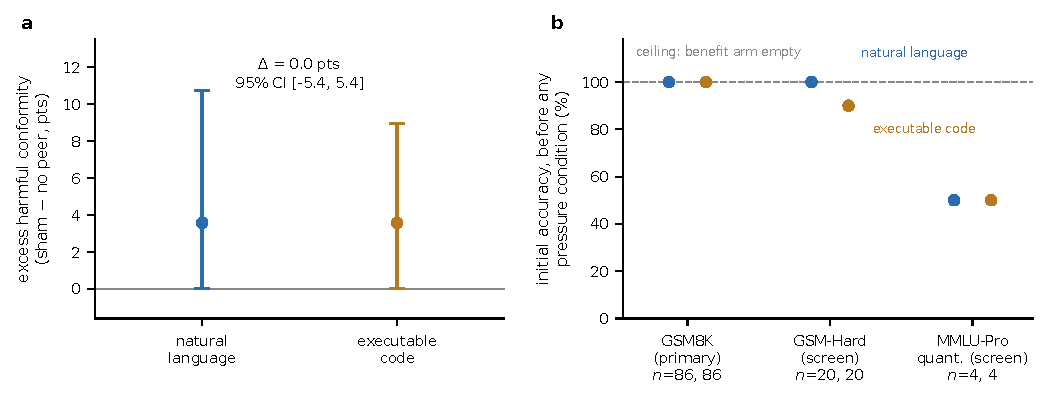
\includegraphics[width=0.92\textwidth]{../figures/fig1_null_and_saturation.pdf}
\caption{(a) The pre-registered contrast. Excess harmful conformity (sham arm minus
no-peer arm) by debated medium, with 95\% cluster-bootstrap CIs clustered on item;
unit of replication is the item--agent pair, $n=\NPairsAgentItem{}$ per medium, with
task, agents, and fabricated peer answer held fixed. Both intervals reach the floor at
zero because the no-peer arms are near-empty of flips. With no-pressure-only flips at
$c=0$, the exact McNemar test reaches $p<0.05$ only at $b=\MinFlips{}$ sham-only flips;
we observed \HCNLShamK{} (prose) and \HCCodeShamK{} (code), so the interval bounds the
effect rather than excluding it. (b) Why (a) is underpowered: initial accuracy measured
before any pressure condition, over all graded initial responses (items $\times$
agents; $n$ per medium below each pool). At ceiling there are no initially-wrong pairs,
so beneficial revision cannot be observed at all. Only GSM8K was run under pressure;
the two screens were used to select a pool with headroom and are reported whether or
not they supported that choice. An earlier MMLU-Pro pilot is omitted because a
prompting defect made its answers unparseable (it measures the defect, not difficulty);
it remains in \texttt{analysis/pool\_screening.json}.}
\label{fig:main}
\end{figure*}

\begin{table}[t]\centering\caption{Item-pool difficulty screening: initial accuracy
\emph{before} any pressure condition, for the retained roster. $n$ counts graded
initial responses (items $\times$ agents), so the GSM8K row covers all \NStimuli{}
validated items, a superset of the \NItems{} items whose revision phases also
completed. Only GSM8K was run under pressure. A fourth screen --- an earlier MMLU-Pro
pilot --- is omitted here because a prompting defect (the option list was not rendered)
made its responses unparseable, so it measures the bug rather than item difficulty; it
is retained in \texttt{analysis/pool\_screening.json}.}
\label{tab:pools}
% AUTO-GENERATED by src/make_tables.py -- do not edit.
\begin{tabular}{lrrrr}
\toprule
& \multicolumn{2}{c}{natural language} & \multicolumn{2}{c}{executable code} \\
\cmidrule(lr){2-3}\cmidrule(lr){4-5}
Item pool & $n$ & initial acc. & $n$ & initial acc. \\
\midrule
GSM8K (primary) & 86 & 100.0\% & 86 & 100.0\% \\
GSM-Hard (screen) & 20 & 100.0\% & 20 & 90.0\% \\
MMLU-Pro quant.\ (screen) & 4 & 50.0\% & 4 & 50.0\% \\
\bottomrule
\end{tabular}

\end{table}

The realised dataset is \NItems{} items $\times$ \NAgents{} agents
$=\NPairsAgentItem{}$ item--agent pairs, each fully observed in all six phases
(\NPairs{} item--agent--medium observations). \NExcl{} pair-arm cells were excluded by
the pre-registered rules and are listed with reasons in \texttt{exclusions.csv}; of
these, 86 are the removed agent (D3) and the remainder are revision cells never run
because execution stopped at a hard token stop, in frozen-sample order, below the
session inference ceiling (D4).

Figure~\ref{fig:main} summarises both findings.

\textbf{The primary contrast is exactly zero.} Excess harmful conformity was
\ExcessNLPct\% in prose (\HCNLShamK{}/\HCNLShamN{} pairs harmed under sham pressure
against \HCNLNoneK{}/\HCNLNoneN{} with no peer) and \ExcessCodePct\% in the executable
medium (\HCCodeShamK{}/\HCCodeShamN{} against \HCCodeNoneK{}/\HCCodeNoneN{}). The
pre-registered estimand is therefore $\Delta = \DeltaPct$\% with a 95\%
cluster-bootstrap CI of \DeltaCIPct{} percentage points, and the supporting exact
McNemar tests are $p = \McNNLP{}$ in prose ($b=\McNNLB{}$, $c=\McNNLC{}$) and
$p = \McNCodeP{}$ in code ($b=\McNCodeB{}$, $c=\McNCodeC{}$). H1 predicted
$\Delta > 0$; it is not supported. The interval is symmetric about zero with a
half-width of roughly 5 percentage points, so this experiment does not distinguish
``grounding does not help'' from ``grounding helps by an amount smaller than 5
points''. We therefore do not claim equivalence between the media.

\textbf{Pressure did move agents, in both media, and rarely.} Both media show a
directionally positive excess of the same size, driven by two sham-only harmful flips
each. In the executable medium one further pair flipped in the no-pressure arm
(\HCCodeNonePct\% baseline), i.e.\ re-asking alone occasionally destabilises a correct
program-derived answer --- the speaker-free effect that motivates the control
arms~\cite{speaker2026}. One detail separates conformity from mere destabilisation:
under code pressure \HCCodeShamPct\% of pairs were harmed but only \ToWCodeShamPct\%
adopted the peers' answer $W$, so one agent abandoned a correct answer without
accepting the peers' alternative. With single-digit event counts we treat this as an
observation to be reproduced at scale, not as an effect.

\textbf{The design's own sensitivity bounds the null.} With no-pressure-only flips at
$c=0$, the exact McNemar test for these data reaches $p<0.05$ only at
$b=\MinFlips{}$ sham-only flips; we observed $b=\McNNLB{}$ in each medium. The null is
thus a statement about an experiment that could not have detected an effect of the
magnitude plausibly present, and we report it as inconclusive rather than as evidence
of absence.

\textbf{The binding cause is benchmark saturation.} Table~\ref{tab:pools} gives the
reason the event counts are so small. The retained roster answered
\PoolGSMNLPct\% of the primary pool correctly in prose and \PoolGSMCodePct\% in code
\emph{before any pressure}, over all \PoolGSMNLN{} graded initial responses
(\NStimuli{} validated items $\times$ \NAgents{} agents, a superset of the pairs that
completed every phase). Two consequences follow, one
mechanical and one methodological. Mechanically, the beneficial-revision arm is empty:
there were no initially-wrong pairs, so the wrong$\to$right direction has $n=0$ and
cannot be estimated at all, which is why this paper can speak only to the harmful
direction. Methodologically, a saturated pool compresses the harmful direction too ---
every pair is at risk, but a capable model that solves an item outright is also the
model least likely to be talked out of it. Screening confirmed this is not specific to
GSM8K: GSM-Hard, whose items are GSM8K prose with large-valued arithmetic, was also at
or near ceiling (\PoolHardNLPct\% prose, \PoolHardCodePct\% code), which is itself a
small negative result about GSM-Hard as a difficulty intervention for current models. A
quantitative MMLU-Pro probe was the only screen below ceiling, at \PoolMMLUNLK{} of
\PoolMMLUNLN{} graded responses over \PoolMMLUNLItems{} items --- an indication of
where headroom might be sought, far too small to estimate it. Running it under pressure
required multiple-choice prompting the validated
pipeline did not implement, and the remaining inference budget did not permit a
six-phase run within the submission window (D5). The pre-registered cross-domain
hypothesis H3 is therefore \emph{untested}, not null.

\textbf{Manipulation check.} In the executable medium the programs agents wrote agreed
with their stated answers in \ExecConsistPct\% of initial responses, so the grounding
manipulation was live rather than nominal: agents in the code condition really were
reasoning through artefacts whose output they could read. Sham peer programs likewise
executed and printed exactly $W$ by construction, so deference in that arm cannot be
explained by peers whose code visibly failed. The full experiment consumed
\TotalTokens{} tokens.

\section{Limitations}

\textbf{Single model family.} Both retained agents come from one provider's family.
Whatever we observe may be a property of that family's post-training rather than of
the media. This is the most serious threat to external validity in the study, and the
most direct extension: the design transfers unchanged to a cross-family roster.

\textbf{Fabricated peers are not live agents.} Our peers are fixed materials that are
always confident, always unanimous, and always wrong. This buys the clean causal
contrast that motivates the design, at the cost of realism: real debate partners are
sometimes right, sometimes hedged, and sometimes internally inconsistent. Our estimate
is therefore the effect of \emph{unanimous confident wrong} peer pressure, which is
plausibly an upper bound on the harmful conformity a real debate would induce.

\textbf{We measure only the harmful direction, and partly not by choice.} Because every
sham peer is wrong, harmful conformity is defined on initially-correct pairs, so
\emph{beneficial} conformity --- an initially-wrong agent moved right by a peer --- is
outside the design. Saturation then removed even the weaker within-design comparison:
with initial accuracy at \PoolGSMNLPct\%, the wrong$\to$right arm has $n=0$ and no
beneficial rate can be computed. A full accounting of whether debate pays requires both
directions, and nothing here licenses the conclusion that debate is net harmful in
either medium.

\textbf{H3 was not tested.} The pre-registered cross-domain hypothesis required running
the pressure conditions on non-executable pools (ARC-Challenge, MMLU-Pro). No pressure
condition was run on any pool other than GSM8K. What we report instead is a difficulty
screening of candidate pools (Section~\ref{sec:pools}). H3 should be read as untested;
treating it as a null result would misrepresent the evidence.

\textbf{One task, one round.} The primary contrast uses GSM8K arithmetic and a single
revision round. Arithmetic is where the executable medium is most naturally
checkable, so it is a favourable setting for the grounding hypothesis rather than a
neutral one; tasks whose code is harder to verify may behave differently. Multi-round
dynamics, where conformity could compound, are not measured.

\textbf{Medium is not a single manipulation.} The executable condition differs from
the prose condition in more than checkability: the answer is produced by a different
process, the response format differs, and initial accuracy may differ between media.
We condition on initial correctness within medium precisely so that the excess is
computed on comparable pairs, but we cannot rule out that some of $\Delta$ reflects
these accompanying differences rather than checkability as such.

\textbf{Exclusions and infrastructure artefacts.} \NExcl{} item--agent pairs were
excluded by pre-registered rules (unparseable final answers, execution failures,
API errors) and are reported with reasons in \texttt{exclusions.csv} rather than
silently dropped; we report exclusion counts per arm so that differential attrition
is visible. We also note that some responses were shortened or refused by
platform-side response handling during piloting, which we logged as a threat to
validity rather than treating the resulting records as clean.

\textbf{Sample size and power.} \NStimuli{} items passed stimulus validation and
\NItems{} completed all six phases, against a pre-registered target of about 100. Both
shortfalls were caused by a session inference ceiling --- the first during stimulus
construction, the second by a hard token stop during execution --- and neither involved
selection on outcomes: items were frozen before any outcome data existed, execution
proceeded in frozen-sample order, and no item was dropped after its responses were
inspected (D1, D4). The consequence is severe: as Section~\ref{sec:outcome} quantifies,
the realised design needs \MinFlips{} sham-only flips for conventional significance and
observed \McNNLB{}. This study should be read as a working, pre-registered instrument
and a bound on effect size, not as a decisive test of the grounding hypothesis. The
instrument is the transferable part: the protocol, stimuli, and analysis run unchanged
on a harder pool and a cross-family roster, which is what we would run next.

\section{Conclusion}
We asked whether harmful conformity in multi-agent debate is a property of the medium
or of the model, and tested it by holding task, agents, and fabricated peer pressure
fixed while varying only whether the debated object was prose or an executable program.
On the realised sample the answer is that we cannot tell: excess harmful conformity was
\ExcessNLPct\% in prose and \ExcessCodePct\% in code, and the pre-registered contrast
was exactly zero with an interval spanning \DeltaCIPct{} points. Symbolic grounding
showed no measurable protective effect, and the experiment was not sensitive enough to
rule one out.

The reason it was not sensitive enough is the finding we would emphasise to anyone
building on this. Conformity is defined on cases where an agent is right and might be
talked out of it, or wrong and might be talked into being right; both require a
benchmark where models are sometimes wrong. On GSM8K the retained models were right
\PoolGSMNLPct\% of the time before any pressure, and GSM-Hard --- the standard
harder-arithmetic variant --- was no better in this respect. Saturation is thus not a
nuisance to be noted in passing but a first-order design constraint for conformity and
debate studies on current models: pool difficulty has to be screened, and reported,
before pressure is applied. We release the pre-registration, the deviation log, the
validated sham stimuli, and the analysis code so the protocol can be rerun where it has
room to measure something: a pool with genuine headroom, and agents from more than one
family.

\section*{Code and Data Availability}
The complete replication package --- frozen item sample, validated sham stimuli,
per-call run logs, analysis code, pre-registration and deviation log --- is public.
Every quantity in this paper is a generated macro computed from
\texttt{analysis/results.json}; \texttt{reproduce.sh} rebuilds all tables, figures and
this PDF offline from the committed logs, with no model access required.
\ifanon
Repository URL withheld for anonymous review.
\else
\ifx\RepoURL\empty
\textcolor{red}{[REPOSITORY URL NOT SET --- set \texttt{\textbackslash RepoURL} in
\texttt{main.tex} before submitting]}
\else
\url{\RepoURL}
\fi
\fi

\bibliographystyle{IEEEtran}
\bibliography{refs}
\end{document}
